\documentclass[a4paper,14pt]{extarticle}
\usepackage[utf8]{inputenc}
\usepackage[russian]{babel}
\usepackage[a4paper, mag=1000, left=2.5cm, right=1cm, top=2cm, bottom=2cm, headsep=0.7cm, footskip=0cm]{geometry}

\title{Анализ плагиата в практических курсах по программированию}
\author{Андрей Цибин, Евгений Ефимчик}
\date{Октябрь 2018}

\usepackage{natbib}
\usepackage{graphicx}
\usepackage{url}
\usepackage{amsmath}
\usepackage{booktabs}

\begin{document}

\maketitle

\begin{abstract}

Проблема недобросовестного заимствования в академической среде по-преж\-нему остается актуальной проблемой. Особо остро она проявляется в среде преддипломного образования. Причинами этому служат многие факторы, в частности, отсутствие преподавания дисциплины научной этики. Недобросовестное заимствование, или плагиат, встречается сегодня в различных формах академической активности, начиная от семестровых работ студентов и заканчивая диссертациями ученых. Отдельной проблемой является недобросовестное заимствование в работах обучающихся учебных заведений, которые они выполняют в рамках практических курсов по программированию. Как и в случае с текстом, выявлять плагиат в ручную является возможным только в самых небольших подвыборках данных. К счастью, на сегодняшний день существует довольно большое количество систем, позволяющих автоматизированно выявлять сходство исходного кода. Более того, существуют средства, позволяющие агрегировать результаты поиска плагиата несколькими различными системами, что также увеличивает вероятность обнаружения случаев недобросовестного заимствования. При этом, данные средства по-прежнему не так распространены, по крайней мере, в отечественных образовательных учреждениях. Вероятно, это вызвано высокой сложностью интерпретации результатов систем анализа плагиата исходного кода.

В настоящей статье, продемонстрирована структура системы анализа плагиата, внедренной в образовательный процесс, а также описан универсальный инструмент интерактивной графовой визуализации результатов анализа плагиата исходного кода.

\end{abstract}

\section{Введение}

Задача выявления плагиата применительно к практическим курсам по программированию становится с каждым годом все более актуальной. Именно по этой причине, в 2017 году на кафедре Компьютерных Образовательных Технологий Университета ИТМО с целью повышения качества автоматизации процесса обучения появилась необходимость в создании автоматизированной системы сдачи и проверки практических заданий по программированию. Изначально, поставленная задача включала в себя автоматизацию процессов проверки работ обучающихся по критериям прохождения ими тестов, оценки качества кода и анализа результатов выявления плагиата.

Система\footnote{Образовательная платформа Flaxo. \url{https://github.com/tcibinan/flaxo}} была разработана в рамках бакалаврской выпускной квалификационной работы \citep{flaxoThesis}, и с начала учебного года 2018-2019 постепенно внедряется в образовательный процесс кафедры.

В следующих разделах описаны составные части модуля анализа плагиата указанной выше системы, а также улучшенный модуль визуализации плагиата.

\section{Инфраструктура}

Концепция оригинальной образовательной платформы включала хранение всех заданий и решений обучающихся в репозиториях системы контроля версий. В частности, в текущем варианте системы существует поддержка системы версионирования Git\footnote{Распределенная система версионирования Git. \url{https://git-scm.com/}}, а в качестве вендора системы - платформа GitHub\footnote{Платформа разработки GitHub. \url{https://github.com/}}, которая на сегодняшний день является одной из самых популярных среди open-source проектов.

Для того чтобы провести анализ существующих решений, необходимо сначала собрать весь исходный код: файлы, написанные преподавателем, которые называются \textit{базовыми}, а также все изменненные или созданные обучающимися. Учитывая, что репозитории с заданиями и решениями помимо исходного кода могут содержать множество других файлов, например, скрипты системы сборки проекта или документацию, необходимо перед выгрузкой заданий и решений фильтровать содержания репозиториев по расширениям файлов. Также загружаемые файлы должны быть сгруппированы по обучающемуся, который их создал или изменил, чтобы дальнейший анализ мог различать автора того или иного фрагмента кода. В качестве временного хранилища исходных файлов можно использовать локальную файловую систему, поскольку количество и размер загружаемых файлов могут быть значительными и не всегда укладываться в объем доступной оперативной памяти.

\section{Инструмент анализа}

Одна из основных задач, возникающая при попытке внедрения системы анализа плагиата это, безусловно, подбор инструментов выявления заимстовований программного кода. На сегодняший день существует значительное количество различных инструментов для этих целей \citep{plagiarismToolsSurvey}. Они различаются механизмом анализа плагиата, форматами входных и выходных данных, скоростью обработки программного кода, а также количеством поддерживаемых языков программирования. Помимо прочего, на основе проанализированной литературы, было установлено, что существует как минимум один инструмент, унифицирующий результаты работы нескольких других инструментов анализа плагиата и предоставляющий более точное значение вероятности плагиата для каждого из случаев\citep{unifiedPlagiarismDetectionTool}.

При разработке настоящего модуля анализа плагиата был выбран инструмент MOSS \citep{mossOriginalPaper}, обладающий рядом характеристик, описанных далее в данном разделе.

MOSS является веб-сервисом анализа плагиата, поддерживающим анализ плагиата на 26 языках программирования. Сервис предоставляет Perl-скрипт в качестве клиентского приложения, который позволяет загружать файлы с исходным кодом и инициализировать анализ плагиата. Наряду с обычными файлами, MOSS использует упомянутое выше понятие базовых файлов. Под этим термином подразумеваются файлы, созданные преподавателем, строки которых должны быть проигнорированы при выявлении заимствованных фрагментов исходного кода.

Как было сказано выше, MOSS принимает на вход набор файлов для анализа, а на выходе генерирует набор HTML-страниц, которые содержат подробные отчеты по каждой паре решений, содержащих заимствованные коды. Отчет включает в себя количество и процент общих строчек всех файлов, а также таблицы с исходным кодом решений, включающие цветовое обозначение общих фрагментов кода. Поскольку формат HTML не пригоден для эффективной автоматической обработки, каждую сгенерированную страницу необходимо самостоятельно парсить и преобразовывать. А учитывая факт, что сервис хранит результаты анализа только 14 суток, после чего удаляет их, необходимо полностью выгружать данные до истечения этого срока.

\section{Визуализация}

\subsection{Графовая визуализация}

Первоначальная версия образовательной платформы Flaxo имела примитивный способ визуализации найденного плагиата: для каждого из обучающихся указывались количество найденных заимствований, а также максимальное значение процента общего кода среди всех найденных заимствований. При этом, если значение последнего превышало некий заданный порог, например 80\%, то в таком случае показатели данного обучающегося выделялись красным цветом, указывая на высокую вероятность недобросовестного заимствования им чужого кода.

Описанный способ визуализации решает свою задачу - он позволяет доступным образом указать преподавателю на работы, которые необходимо проверить в первую очередь, а какие с меньшей вероятностью обладают заимствованиями. Однако, подобная система визуализации не может дать преподавателю полной картины происходящего, поскольку она не указывает на закономерности, которые определяются более чем двумя работами. Действительно, механизм анализа плагиата предполагает попарное сравнение всех работ обучающихся, поэтому выявление небинарных зависимостей может оказаться непростой задачей. При этом, подобные зависимости, могут выявлять, например, группы недобросовестных обучающихся, которые делятся друг с другом своим исходным кодом. При этом, если похожие заимствования имеются более чем у двух людей, то это значительно уменьшает вероятность ложного срабатывания системы анализа плагиата.

Одним из возможных способов представления данных, позволяющим наблюдать сложные зависимости, является графовая визуализация. На сегодняшний день существует, как минимум один инструмент графовой визуализации результатов анализа плагиата \citep{plagiarismGraph}. Как показано в связанной статье, использование графов для отображения результатов анализа плагиата наравне с гистограммами распределения процента заимствованного кода, повышает эффективность примения системы анализа плагиата в целом. Кроме того, использование наложеных графовых представлений нескольких заданий в практических курсах, позволяет свести на нет влияние ложных срабатываний алгоритма анализа плагиата. При таком подходе становится возможным выявлять группы обучающихся, которые стабильно выделяются на фоне своих коллег и тем самым, вероятнее всего, действительно недобросовестно используют чужой исходный код.

Использование графов для отображения результатов анализа плагиата даже одного задания в отдельности, с точки зрения наглядности, имеет очевидные преимущества перед табличным представлением.

\subsection{Инструмент графовой визуализации}

Упомянутый выше инструмент визуализации плагиата делает большой шаг вперед к простоте интерпретации результатов анализа плагиата. Однако, система не позволяет динамически менять параметры, определяющие структуру графа, что ограничивает преподавателя в возможности наглядного рассмотрения зависимостей в различных перспективах и с отличающимся масштабом. По этой причине в рамках настойщей работы был создан универсальный инструмент\footnote{Универсальный инструмент интерактивной визуализации графов. \url{https://github.com/tcibinan/graph2viz}} интерактивной визуализации графов.

Инструмент рассматривает обучающихся как вершины графа, а случаи заимствования как ребра графа, соединяющие двух различных обучающихся. В качестве веса ребра $w$ используется значение процента соответствующего заимствования, которое лежит в полуинтервале $(0,100]$. Учитывая, что б\'{о}льшие веса соответствуют меньшим расстояниям между двумя решениями в пространстве всех возможных решений некоторой задачи, необходимо в качестве длин ребер $l$ использовать значения обратно пропорциональные их весу. При таком подходе на построенном графе можно визуально различать кластеры, каждый из которых определяет группу обучающихся, работы которых содержат значительно выделяющееся количество заимствований друг между другом. В случае отсутствия ярко выделенных кластеров, можно говорить о том, что примеров плагиата в работах найти не удалось или о том, что необходимо изменить параметры отображения графа.

В рамках проведения двух практических курсов по программированию на языке Java, включающем в общем сложности 12 заданий, с использованием оригинальной платформы было отмечено следующее явление: норма распределения процентов заимствованного кода для каждого задания уникальна и может значительно отличаться. При этом, низкий процент заимствонного кода в части заданий с нормой распределения, смещенной к нулю, не обязательно означает сниженный уровень заимствования кода в этом задании. 

Предположительно, в описанных случаях имеет смысл нормализовать веса, чтобы они укладывались в интервал $[0, 1]$, причем правой границей должен соответствовать максимальный вес ребер из представленных. Для некоторых заданий, однако, подобный подход может оказаться непригодным и стоит нормализовывать веса так, чтобы правой границе интервала соответствовали ребра с весом равным 100. Следовательно, инструмент должен иметь возможность поддержки нескольких типов нормализации.

Дополнительный интерес представляет возможность \textit{пороговой нормализации}, которая бы позволяла объединять в кластеры только таких обучающихся, у которых как минимум один из процентов заимствованного кода выше некоторого заданного порогового значения $r$.

Помимо прочего, существует ряд случаев, ведущих к необходимости как относительного, так и абсолютного масштабирования длин ребер графа. К примеру, при отключенной нормализации весов задания со смещенной нормой распределения процентов заимствованного кода влево будут представлены графом с очень короткими ребрами, на котором крайне сложно разобрать отдельные связи. В этом случае существование относительного масштабирования позволит сохранить пропорции длин ребер и при этом сделать их различимыми. В другом случае, при очень высоких значениях весов ребер, их длины стремятся к нулю, отчего вершины графа могут накладываться друг на друга и становиться трудноразличимыми. Возможность абсолютного масштабирования позволяет справиться с этой ситуацией, путем добавления некоторой фиксированой базовой длины всем ребрам.

Итоговая формула длины ребра графа представляется в следующем виде
\begin{equation}
    l_i = (1-\eta(w_i))s+h \text{ для всех i} \in 1, ..., n,
\end{equation}
где $l_i$ - длина $i$-ого ребра,
\\$w_i$ - вес $i$ ребра,
\\$n$ - число ребер в графе,
\\$\eta$ - выбранная функция нормализации,
\\$s$ - параметр относительного масштабирования,
\\$h$ - параметр абсолютного масштабирования.

Перечень функций нормализации представлен в таблице \ref{tab:normalization}.

\begin{table}[htb]
    \centering
    \begin{tabular}{lc}
        \toprule
            Стандартная &
            \(\displaystyle
                \eta(w) = w / 100
            \)\\
        \midrule
            Адаптивная &
            \(\displaystyle
                \eta(w) = w / \max_{1 \leq i \leq n}{w_i}
            \)\\
        \midrule
            Пороговая &
            \(\displaystyle
                \eta(w) = 
                \begin{cases}
                    1 &\text{при } w \geq r,\\
                    0 &\text{при } w < r
                \end{cases}
            \)\\
        \bottomrule
    \end{tabular}
    \caption{Функции нормализации}
    \label{tab:normalization}
\end{table}

\section{Пайплайн анализа плагиата}

На этапе, когда определены промежуточные этапы, необходимые для проведения анализа плагиата в практическом курсе по программированию, можно описать целостное представление модуля анализа плагиата. Все стадии анализа схематично представлены на рис. \ref{fig:pipeline}.

\begin{figure}[h!]
\centering
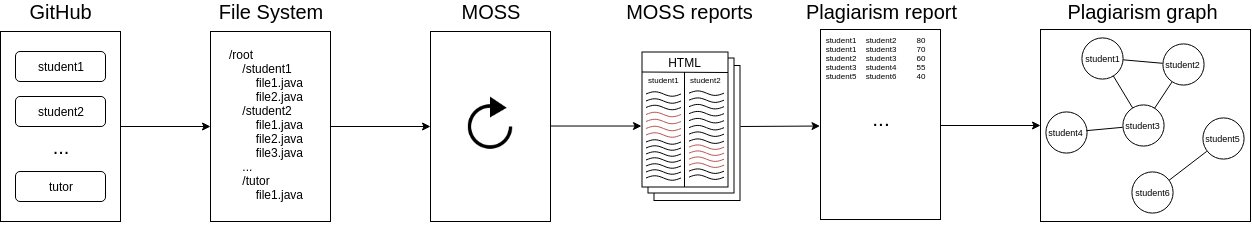
\includegraphics[width=1.0\textwidth]{graph2viz.png}
\caption{Стадии анализа плагиата}
\label{fig:pipeline}
\end{figure}

Построенный пайплайн анализа плагиата задания практического курса по программированию включает следующие шаги:
\begin{enumerate}
    \item агрегацию задания и решений,
    \item загрузку задания и решений на сервер MOSS,
    \item выгрузку всех результатов, сгенерированных MOSS,
    \item составление отчета по результатам анализа плагиата,
    \item генерацию графа заимствований.
\end{enumerate}

Результатом работы описанного пайплайна анализа плагиата является отображение динамически конфигурируемого графа заимствований, пример которого приведен на рис. \ref{fig:graph}. При необходимости преподаватель может менять значения параметров масштабирования длин ребер графа, порогового значения веса отображаемых ребер, и, кроме того, он может выбирать применяемую функцию нормализации. На каждое действие пользователя граф меняет свои параметры и плавно переходит в требуемое состояние.

\begin{figure}[h!]
\centering
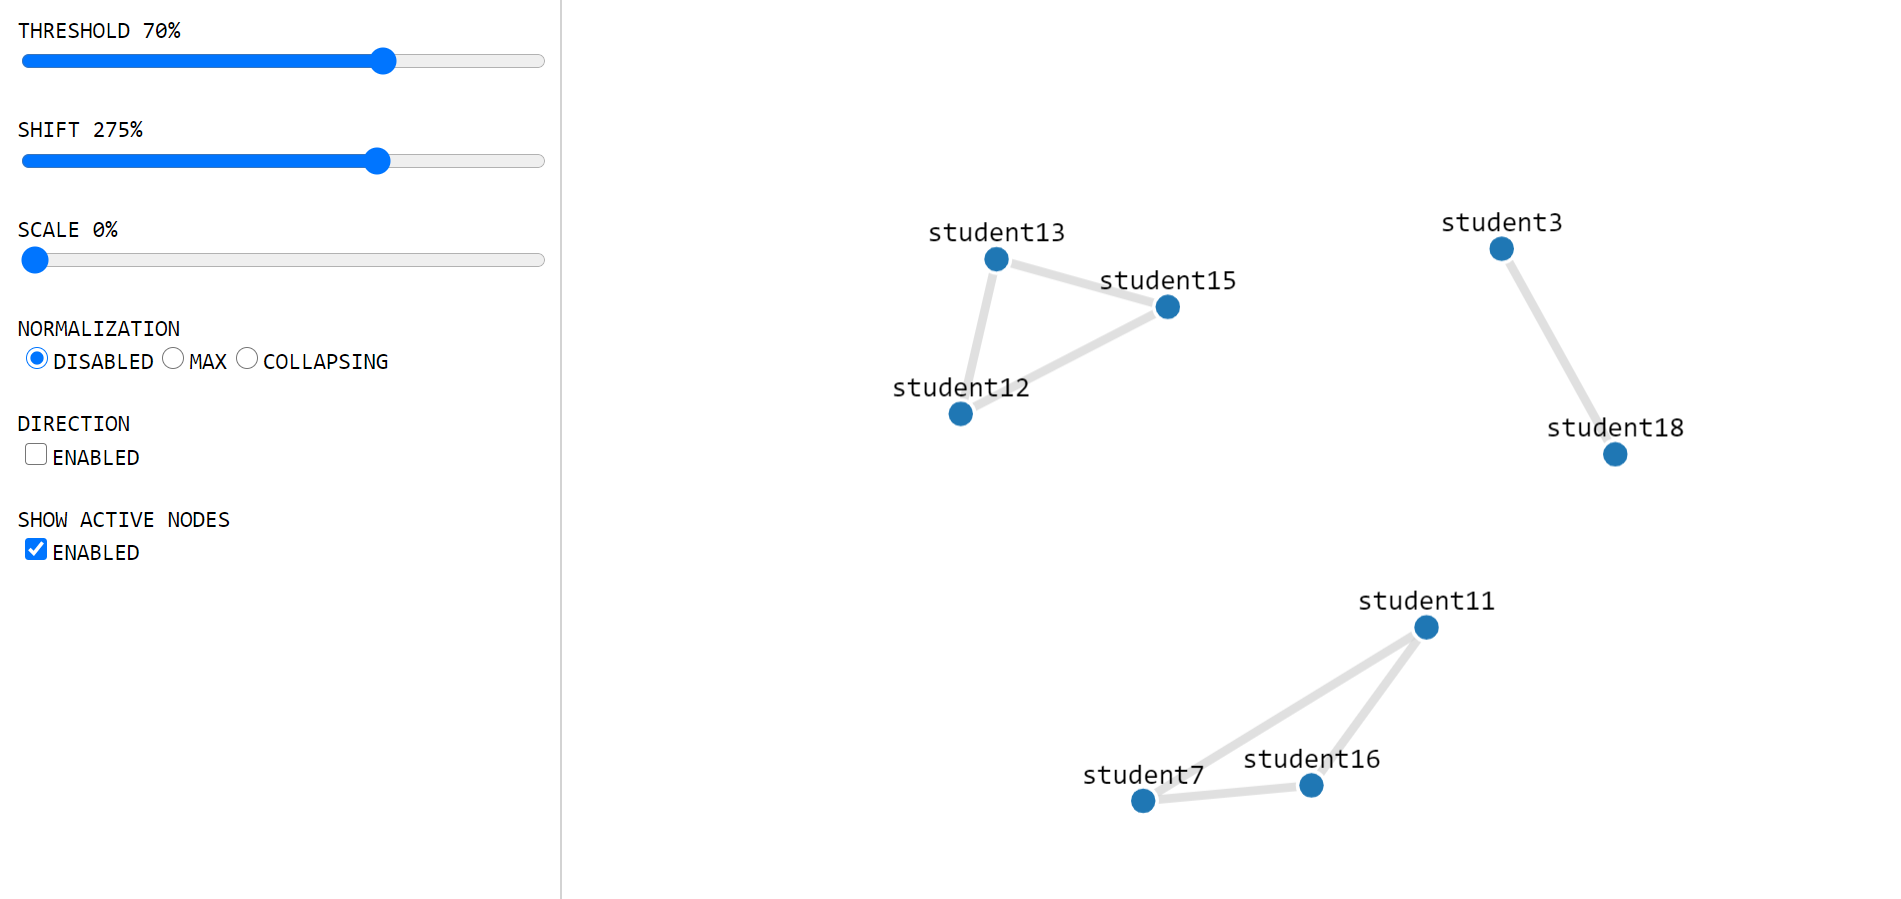
\includegraphics[width=1.0\textwidth]{graph.png}
\caption{Граф заимствований}
\label{fig:graph}
\end{figure}

\section{Дальнейшее развитие}

На текущий момент представленный модуль анализа плагиата и, в частности, инструмент графовой визуализации, обладает значительным потенциалом с точки зрения наглядности представления результатов анализа плагиата. В то же время, на сегодняшний момент еще не собрана формализованная информация о качественных результах внедрения данного модуля в образовательный процесс. Сбор информации осуществляется в настоящий момент.

Кроме того, построенный пайплайн анализа плагиата в практических курсах обладает рядом ограничений. Во-первых, не вся информация, которую генерирует MOSS, предоставляется преподавателю в адаптированном виде. Например, информация о конкретных совпадениях строчек кода между двумя решениями представлена в изначальном виде, наглядность которого потенциально может быть улучшена. Во-вторых, визуализация на текущий момент учитывает данные об анализе плагиата только одного единственного задания. При этом, как было отмечено ранее в настоящей работе, наложение результатов анализа плагиата нескольких заданий положительно влияет на качество финального результат. В-третьих, на текущий момент визуализация результатов анализа плагиата представляется лишь одним из возможных подходов - графовым отображением. Однако, поддержка иных видов визуализации может улучшить наглядность результатов работы модуля анализа плагиата в целом.

\section{Заключение}

Поскольку применение автоматизированных средств анализа плагиата в работах обучающихся становится сегодня обыденностью, модуль анализа плагиата подобный описанному в настоящей работе может оказаться незаменимым инструментом, который помогает преподавателю контролировать добросовестность обучающихся.

При этом крайне важно понимать, что никакой инструмент анализа плагиата не может дать точных гарантий и однозначно указать на случаи недобросовестного заимствования. Инструменты могут лишь указывать направление для изучения и анализа, но они не должны быть главенствующим фактором, который бы учитывался слепо и непосредственно влиял на судьбу того или иного обучающегося, заподозренного в недобросовестном заимствовании. В конечном счете, решения должны приниматься людьми и каждый случай должен рассматриваться персонально.

\bibliographystyle{plain}
\bibliography{references}
\end{document}
